\section{Zustandsreglerentwurf} \label{sec:Zustandsreglerentwurf}

\subsection{Einfache Zustandsrückführung} \label{sec:Ackermann-Formel}

Die erste umgesetzte Regelstrategie ist die einfache Zustandsrückführung unter Anwendung der Ackermann-Formel für Systeme mit einem Eingang. Ziel ist es, das Pendel-System mit einem Anfangswinkel ungleich Null Grad erneut in die instabile Ruhelage zu bringen. Dafür werden mit Hilfe der Ackermann-Formel k-Faktoren berechnet, welche anschließend mit den Zuständen $x_{\mathrm{1}}$ bis $x_{\mathrm{4}}$ multipliziert und auf den Systemeingang zurückgeführt werden (\autoref{fig:Bild7}). Der Wagen wird dabei immer in den Ausgangszustand von $x_{\mathrm{M}}$ zurück geregelt.

\begin{figure}[H]
    \centering
    \fbox{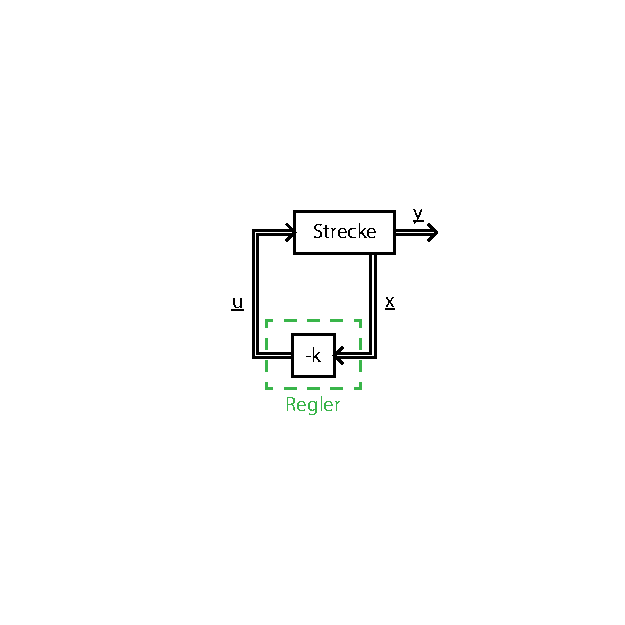
\includegraphics[width=0.3\textwidth]{Bilder/Ackermann.pdf}}
    \caption[Reglerstruktur einfache Zustandsrückführung]{Schematische Darstellung der Reglerstruktur der einfachen Zustandsrückführung}
    \label{fig:Bild7}
\end{figure}

Im ersten Schritt wird der Nachweis der Steuerbarkeit des Systems benötigt. Dieser wurde bereits in \autoref{sec:Steuerbarkeit} erbracht.
Im zweiten Schritt erfolgt die Bestimmung der Eigenwerte der Systemmatrix A. Hierzu wird das charakteristische Polynom benötigt, welches mithilfe der Laplace-Transformation der Vektorzustandsdifferentialgleichungen $\underline{\dot{x}}$ und der anschließenden Umformung hergeleitet wird.\\\\
Laplace-Transformation und Umformung:
\begin{align*}
    \underline{\dot{x}} &= \underline{A}\cdot\underline{x}+\underline{B}\cdot\underline{u}\quad\laplace \quad s\cdot \underline{X}(s)-\underline{x}_{\mathrm{0}}=\underline{A}\cdot \underline{X}(s)+\underline{B}\cdot \underline{U}(s) \\
    \underline{X}(s) &= (s\cdot \underline{I} - \underline{A})^{-1}\cdot\underline{x}_{\mathrm{0}}+(s\cdot \underline{I} - \underline{A})^{-1}\cdot\underline{B}\cdot\underline{U}(s)
\end{align*}
\newline
Das charakteristische Polynom folgt aus der Determinante von: ($s\cdot\underline{I}-\underline{A}$). Die Matrix $\underline{I}$ stellt die Einheitsmatrix dar. Die Nullstellen des Polynoms gleichen den Eigenwerte der Systemmatrix A.

\clearpage

Charakteristische Polynom und Eigenwertdefinition:
\begin{align*}
    \underline{P}(s) &= det(s\cdot\underline{I}-\underline{A}) \\
    \underline{P}(s_{\mathrm{P}}) &= \underline{0} = eig(\underline{A})
\end{align*}
\newline
Allgemeine Form:
\begin{align*}
        \underline{P}(s) &= s^n+\alpha_{n-1}\cdot s^{\mathrm{n-1}}+...+\alpha_{\mathrm{1}}\cdot s + \alpha_{\mathrm{0}} \\
        \underline{P}(s) &= (s-s_{\mathrm{P1}})\cdot(s-s_{\mathrm{P2}})\cdot ... \cdot (s-s_{\mathrm{Pn}})
\end{align*}
\newline
Die Berechnung der Eigenwerte der Systemmatrix erfolgt analog zu den vorangegangenen Betrachtungen.\\\\
Eigenwerte des Systems:
\begin{align}\label{eq:Gleichung36}
    eig(\underline{A}) &= eig
    \begin{bmatrix}
        0 & 1 & 0 & 0 \\
        26.6505 & -0.0248 & 0 & 5.8333 \\
        0 & 0 & 0 & 1 \\
        -0.8502 & 7.916\cdot10^-4 & 0 & -2.333
    \end{bmatrix} \nonumber\\
    eig(\underline{A}) &=
    \begin{bmatrix}
        0 \\
        5.0852 \\
        -5.3333 \\
        -2.1100
    \end{bmatrix}
\end{align}
\newline
Die Eigenwerte müssen einen negativen Realteil aufweisen, andernfalls ist das System instabil. Die Polstellen des Reglers werden auf $s_{\mathrm{P}} = -4+0j$ festgelegt. Die Lage aller Polstellen ist in \autoref{fig:Bild8} visualisiert.\\\\
Reglerpolstellen:
\begin{align}\label{eq:Gleichung37}
    \underline{s}_{\mathrm{P}} &= 
    \begin{bmatrix}
        -4 & -4 & -4 & -4 
    \end{bmatrix}
\end{align}

\begin{figure}[H]
    \centering
    \fbox{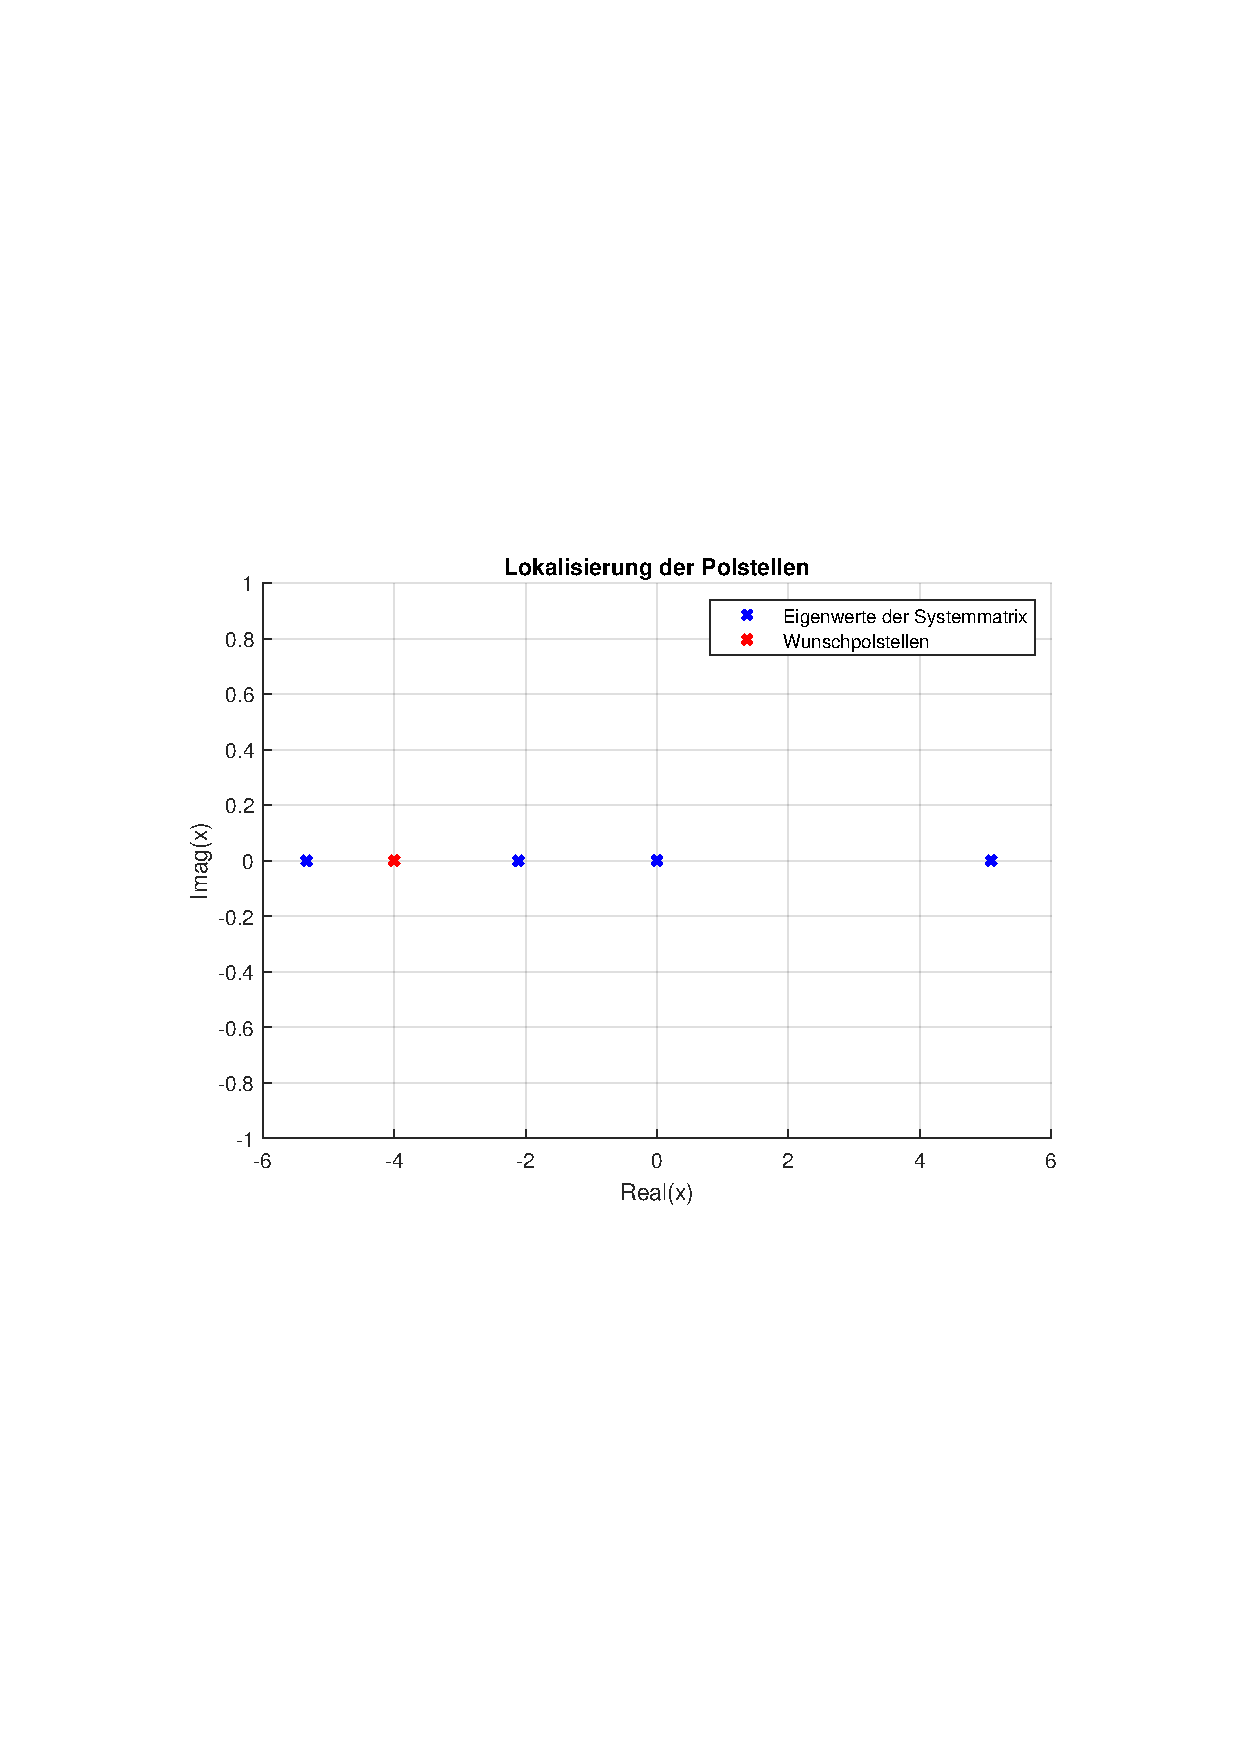
\includegraphics[width=0.75\textwidth]{Bilder/Polstellen_Ackermann.pdf}}
    \caption[Polstellenlage einfacher Zustandsregler]{Polstellenlagen des Systems mit einfachen Zustandsregler}
    \label{fig:Bild8}
\end{figure}

Zur Bestimmung der Koeffizienten $\alpha_{\mathrm{n}}$ bis $\alpha_{\mathrm{0}}$ des geregelten Systems, wird das charakteristische Polynom ausmultipliziert und die Wunschpolstellen eingesetzt.\\\\
Berechnung der Koeffizienten:
\begin{align*}
    \underline{P}(s) &= (s-s_{\mathrm{P1}})\cdot(s-s_{\mathrm{P2}})\cdot(s-s_{\mathrm{P3}})\cdot(s-s_{\mathrm{P4}}) \\
    \underline{P}(s) &= s^4-s^3\cdot(s_{\mathrm{P1}}+s_{\mathrm{P2}}+s_{\mathrm{P3}}+s_{\mathrm{P4}}) \nonumber \\ 
    &\quad +s^2\cdot(s_{\mathrm{P1}}\cdot(s_{\mathrm{P2}}+s_{\mathrm{P3}}+s_{\mathrm{P4}})+s_{\mathrm{P2}}\cdot(s_{\mathrm{P3}}+s_{\mathrm{P4}})+s_{\mathrm{P3}}\cdot s_{\mathrm{P4}}) \nonumber \\
    &\quad -s\cdot(s_{\mathrm{P1}}\cdot(s_{\mathrm{P2}}\cdot s_{\mathrm{P3}}+s_{\mathrm{P2}}\cdot s_{\mathrm{P4}}+s_{\mathrm{P3}}\cdot s_{\mathrm{P4}})+s_{\mathrm{P2}}\cdot s_{\mathrm{P3}}\cdot s_{\mathrm{P4}}) \nonumber \\
    &\quad +(s_{\mathrm{P1}}\cdot s_{\mathrm{P2}}\cdot s_{\mathrm{P3}}\cdot s_{\mathrm{P4}})
\end{align*}
\newline
Das charakteristische Polynom und die Koeffizienten folgen zu:
\begin{align}
    \underline{P}(s) &= s^4+16\cdot s^3+96\cdot s^2+256\cdot s+256 \nonumber \\
    \underline{\alpha} &=
    \begin{bmatrix}
        256 & 256 & 96 & 16 & 1
    \end{bmatrix} \label{eq:Gleichung38}
\end{align}
\newline
Zur Berechnung der Verstärkungsfaktoren des Reglers wird die letzte Zeile $t_{\mathrm{n}}^T$ der inversen Steuerbarkeitsmatrix $Q_{\mathrm{s}}^{-1}$ benötigt.\\\\
Inverse Steuerbarkeitsmatrix $Q_{\mathrm{s}}^{-1}$:
\begin{align*}
    \underline{Q}_{\mathrm{s}}^{-1} &=
    \begin{bmatrix}
         0 & -0.8333 & 1.9651 & -26.7984 \\
        -0.8333 & 1.9651 & -26.7984 & 67.7740 \\
        0 & 0.3333 & -0.7784 & 2.5264 \\
        0.3333 & -0.7784 & 2.5264 & -7.5869
    \end{bmatrix}^{-1} \\
    \underline{Q}_{\mathrm{s}}^{-1} &=
    \begin{bmatrix}
        0 & -0.1040 & 7 & 3.26 \\
        -0.1092 & -0.1142 & 3.2665 & 0.2854 \\
        -0.1165 & -0.0488 & 0.2885 & 0.1221 \\
        -0.0489 & 0 & 0.1223 & -0.0001
    \end{bmatrix}
\end{align*}
\newline
Letzte Zeile der inversen Matrix:
\begin{align} \label{eq:Gleichung39}
    \underline{t}_{\mathrm{4}}^T &=
    \begin{bmatrix}
        -0.0489 & 0 & -0.1223 & -0.0001
    \end{bmatrix}
\end{align}
\newline
Die finale Berechnung erfolgt auf Grundlage der \autoref{eq:Gleichung40}. Durch das Einsetzen der letzten Zeile der inversen Steuerbarkeitsmatrix (\autoref{eq:Gleichung39}), der Faktoren aus \autoref{eq:Gleichung38} und der Systemmatrix A folgt für die Verstärkungsfaktoren $\underline{k}^T_{\mathrm{Acker}}$ der Zustandsrückführung:
\begin{align}
    \underline{k}^T &= \underline{t}_{\mathrm{n}}^T\cdot(\alpha_{\mathrm{0}}\cdot\underline{I} + \alpha_{\mathrm{1}}\cdot \underline{A} + ... + \alpha_{\mathrm{n-1}}\cdot \underline{A}^{n-1}+\underline{A}^n) \label{eq:Gleichung40}\\
    \underline{k}^T_{\mathrm{Acker}} &=
    \begin{bmatrix}
        -159.9929 & -31.7079 & -31.3150 & -38.3441
    \end{bmatrix} \label{eq:Gleichung41}
\end{align}

\subsection{Vorsteuerung}

Mithilfe des Vorfilters können Referenzpositionen für die Systemzustände vorgegeben werden. Im weiteren Verlauf wird lediglich eine Referenzposition des Wagens vorgegeben, d.h. der Wagen fährt während des Pendelschwingens eine Endlage abweichend zum Ursprung an. Der Referenzwert wird auf den Systemeingang gegeben. Dieser wird anschließend mit dem Vorfilter $\underline{F}$ multipliziert. Weiterhin erfolgt die Verrechnung mit den Faktoren $\underline{k}$, welche analog zum \autoref{sec:Ackermann-Formel} berechnet werden (\autoref{fig:Bild9}).\\\\
Eingangsgleichung des Systems:
\begin{align}\label{eq:Gleichung42}
    \underline{u}(t) &= -\underline{k}\cdot\underline{x}(t)+\underline{F}\cdot\underline{y}_{ref}(t)
\end{align}

\begin{figure}[H]
    \centering
    \fbox{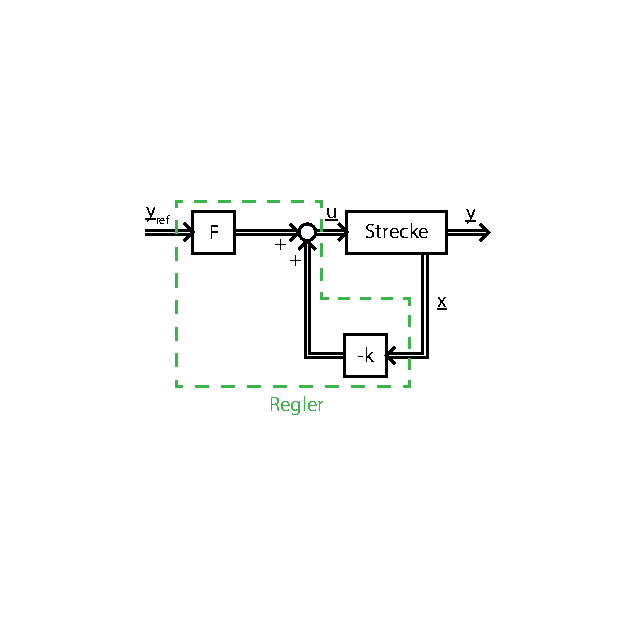
\includegraphics[width=0.5\textwidth]{Bilder/Vorsteuerung.pdf}}
    \caption[Reglerstruktur Vorsteuerung]{Schematische Darstellung der Reglerstruktur der Referenzwert-Vorsteuerung}
    \label{fig:Bild9}
\end{figure}

Zur Ermittlung der Matrix $\underline{F}$ des Vorfilters werden zuerst die im Zeitbereich geltenden Kriterien aufgestellt. Der Ausgang des Systems $\underline{y}(t)$ muss nach unendlicher Zeit $t$ in den Referenzwert $\underline{y}_{ref}$ laufen. Der Referenzwert wird als konstant angenommen.\\\\
Kriterien im Zeitbereich:
\begin{align}
    \lim_{t \to \infty} \underline{y}(t) &= \underline{y}_{ref} = \underline{y}_{0ref} = const. \label{eq:Gleichung43}\\
    \underline{y}_{ref}(t) &=
    \begin{cases}
        \underline{y}_{0ref} & t \geq 0 \\
        0 & \, \text{sonst}
    \end{cases} \label{eq:Gleichung44}
\end{align}
\newline
Da die Berechnungen im Zeitbereich aufwendig sind, werden weitere Betrachtungen im Laplace-Bereich vorgenommen. Vorteil der Transformation ist das Rechnen mit algebraischen Gleichungen. Zur Überführung des Ansatzes aus \autoref{eq:Gleichung43} wird der Grenzwertsatz der Laplace-Transformation angewandt. Das Referenzzeitsignal $\underline{y}_{ref}(t)$ aus \autoref{eq:Gleichung44} wird ebenfalls überführt.\\\\
Grenzwertsatz der Laplace-Transformation und Überführung des Referenzzeitsignals:
\begin{align}
    \lim_{t \to \infty} \underline{y}(t) &= \lim_{s \to 0} s\cdot\underline{Y}(s) = \underline{y}_{ref} = \underline{y}_{0ref} \label{eq:Gleichung45}\\
    \underline{Y}_{ref}(s) &= \frac{1}{s}\cdot\underline{y}_{0ref} \label{eq:Gleichung46}
\end{align}
\newline
Für weitere Betrachtungen wird das Zustandsraummodell der Strecke in den Laplace-Bereich transformiert.

\clearpage

Laplace-Transformation der Strecke:
\begin{align}
    \underline{\dot{x}}(t) &= \underline{A}\cdot\underline{x}+\underline{B}\cdot\underline{u}(t)\quad\laplace\quad s\cdot \underline{X}(s) = \underline{A}\cdot\underline{X}(s)+\underline{B}\cdot\underline{U}(s) \label{eq:Gleichung47}\\
    \underline{y}(t) &= \underline{C}\cdot\underline{x}(t) \quad\laplace\quad \underline{Y}(s) = \underline{C}\cdot\underline{X}(s) \label{eq:Gleichung48}
\end{align}
\newline
Die \autoref{eq:Gleichung47} wird nach $\underline{X}(s)$ umgestellt und entsprechend in die Laplace-transformierte Ausgangsgleichung $\underline{Y}(s)$ eingesetzt. Aus der Umstellung geht hervor, dass das System durch eine Multiplikation aus einer Übertragungsfunktion $\underline{G}(s)$ und dem Eingangssignal $\underline{U}(s)$ gebildet werden kann.\\\\
Umformungen:
\begin{align}
    \underline{B}\cdot\underline{U}(s) &= (s\cdot\underline{I}-\underline{A})\cdot\underline{X}(s) \label{eq:Gleichung49}\\
    \underline{X}(s) &= (s\cdot\underline{I}-\underline{A})^{-1}\cdot\underline{B}\cdot\underline{U}(s) \nonumber \\
    \underline{Y}(s) &= \underline{C}\cdot(s\cdot\underline{I}-\underline{A})^{-1}\cdot\underline{B}\cdot\underline{U}(s) \label{eq:Gleichung50}\\
    \underline{G}(s) &= \underline{C}\cdot(s\cdot\underline{I}-\underline{A})^{-1}\cdot\underline{B} \nonumber
\end{align}
\newline
Die Eingangsgleichung des Systems (\autoref{eq:Gleichung42}) wird transformiert und anschließend in \autoref{eq:Gleichung49} eingesetzt.\\\\
Laplace-Transformation der Eingangsgleichung:
\begin{align*}
    \underline{U}(s) &= -\underline{k}\cdot\underline{X}(s)+\underline{F}\cdot\underline{Y}_{\mathrm{ref}}(s)
\end{align*}
\newline
Einsetzen und Umformung nach $\underline{X}(s)$:
\begin{align}
    \underline{B}\cdot(\underline{F}\cdot\underline{Y}_{\mathrm{ref}}(s)-\underline{k}\cdot\underline{X}(s)) &= (s\cdot\underline{I}-\underline{A})\cdot\underline{X}(s) \nonumber \\
    \underline{B}\cdot \underline{F}\cdot\underline{Y}_{\mathrm{ref}}(s) &= (s\cdot\underline{I}-\underline{A}+\underline{B}\cdot{\underline{k}})\cdot\underline{X}(s) \nonumber \\
    \underline{X}(s) &= (s\cdot\underline{I}-\underline{A}+\underline{B}\cdot{\underline{k}})^{-1}\cdot\underline{B}\cdot \underline{F}\cdot\underline{Y}_{\mathrm{ref}}(s) \label{eq:Gleichung51}
\end{align}
\newline
Die \autoref{eq:Gleichung51} wird in \autoref{eq:Gleichung48} eingesetzt, um die Übertragungsfunktion des geschlossenen Regelkreises zu erhalten.

\clearpage

Übertragungsfunktion des geschlossenen Regelkreises:
\begin{align}
        \underline{Y}(s) &= \underline{C}\cdot(s\cdot\underline{I}-\underline{A}+\underline{B}\cdot{\underline{k}})^{-1}\cdot\underline{B}\cdot F\cdot\underline{Y}_{\mathrm{ref}}(s) \label{eq:Gleichung52}
\end{align}
\newline
Aus der vorangegangenen Betrachtung ist nur die Matrix $\underline{F}$ des Vorfilters unbekannt. Um dasjenige $F$ zu ermitteln, welches die stationäre Exaktheit erfüllt, wird der Grenzwertsatz aus \autoref{eq:Gleichung45} angesetzt und die Übertragungsfunktion des geschlossenen Regelkreises (\autoref{eq:Gleichung52}) eingesetzt.\\\\
Stationäre Exaktheit:
\begin{align}
    \lim_{s \to 0} s\cdot \underline{Y}(s) &= \underline{y}_{0ref} \nonumber \\
    \lim_{s \to 0} s\cdot (\underline{C}\cdot(s\cdot\underline{I}-\underline{A}+\underline{B}\cdot{\underline{k}})^{-1}\cdot\underline{B}\cdot\underline{F}\cdot\frac{1}{s}\cdot\underline{y}_{0ref}) &= \underline{y}_{0ref} \label{eq:Gleichung53}
\end{align}
\newline
Nach dem Vereinfachen der \autoref{eq:Gleichung53} geht hervor, dass der Term $\underline{C}\cdot(-\underline{A}+\underline{B}\cdot{\underline{k}})^{-1}\cdot\underline{B}\cdot\underline{F}$ der Einheitsmatrix $\underline{I}$ gleichen muss (\autoref{eq:Gleichung54}). Andernfalls ist die Gleichung nicht erfüllbar. Durch die Kenntnis kann die Matrix $\underline{F}$ des Vorfilters bestimmt werden (\autoref{eq:Gleichung55}).\\\\
Umstellung nach $\underline{F}$:
\begin{align}
    \underline{C}\cdot(-\underline{A}+\underline{B}\cdot{\underline{k}})^{-1}\cdot\underline{B}\cdot\underline{F} &= \underline{I} \label{eq:Gleichung54}\\
    \underline{F} = (\underline{C}\cdot(-\underline{A}+\underline{B}\cdot{\underline{k}})^{-1}\cdot\underline{B})^{-1} \label{eq:Gleichung55}
\end{align}
\newline
Die Anwendbarkeit des Reglergesetztes ist eingeschränkt, da nur quadratische Matrizen invertierbar sind. Die Dimensionen der einzelnen Matrizen lauten wie folgt:

\begin{itemize}
    \item $A\in\mathbb{R}^{(nxn)}$
    \item $B\in\mathbb{R}^{(nxm)}$
    \item $C\in\mathbb{R}^{(pxn)}$
    \item $k\in\mathbb{R}^{(mxn)}$
\end{itemize}

Die Matrix $\underline{F}$ ist quadratisch, sobald $p = m$ gilt, d.h. die Anzahl der Systemeingänge muss gleich der Anzahl der Systemausgänge sein, d.h. die benötigte C-Matrix zur Berechnung des Vorfilters lautet: $C = [0\quad 0\quad 1\quad 0]$.
Die Polstellen der Reglerstuktur werden folgendermaßen festgelegt.

\clearpage

Reglerpolstellen:
\begin{align}\label{eq:Gleichung56}
    \underline{s}_{P} &=
    \begin{bmatrix}
        -4.5 & -4.5 & -4.5 & -4.5
    \end{bmatrix}
\end{align}
\newline
Die Polstellenlagen sind in \autoref{fig:Bild10} dargestellt.

\begin{figure}[H]
    \centering
    \fbox{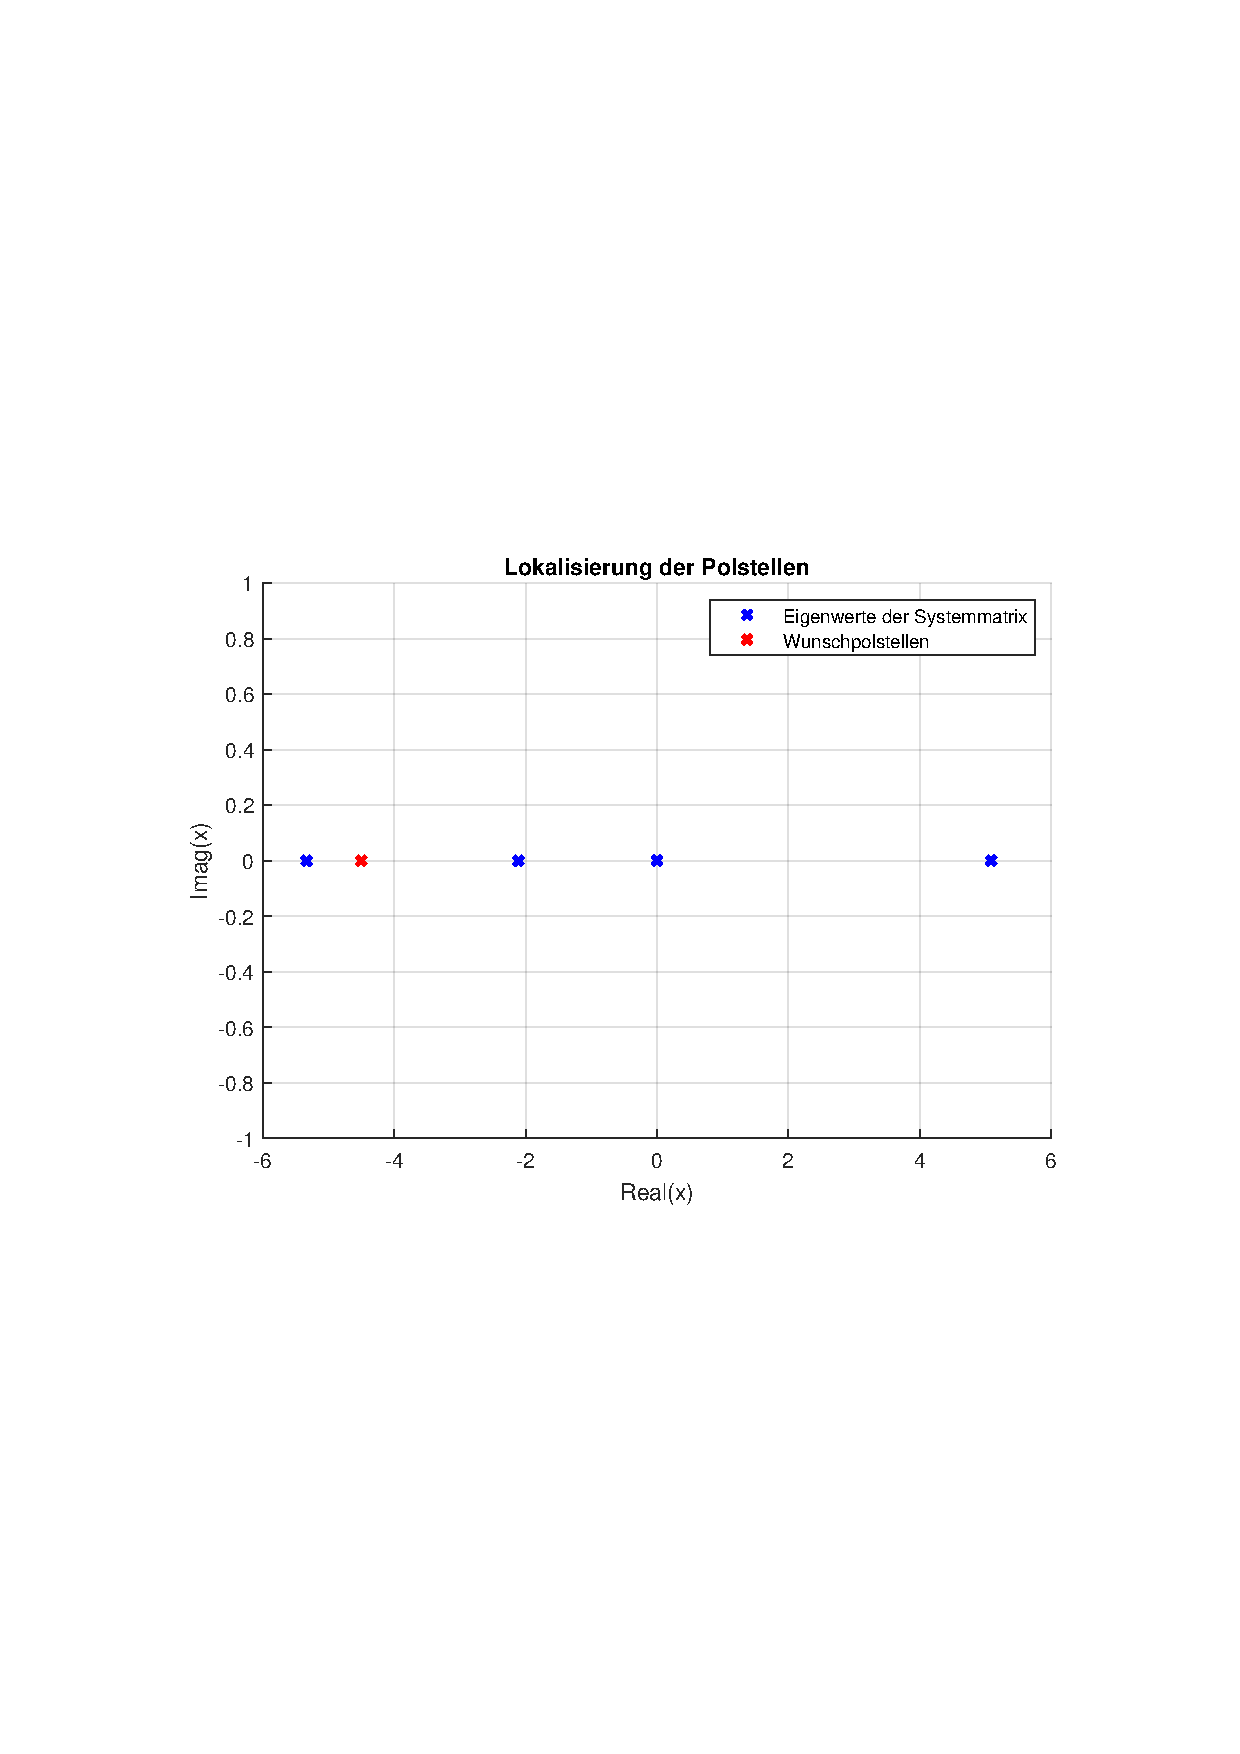
\includegraphics[width=0.75\textwidth]{Bilder/Polstellen_Vorsteuerung.pdf}}
    \caption[Polstellenlage Vorsteuerung]{Polstellenlagen des Systems mit Referenzwert-Vorsteuerung}
    \label{fig:Bild10}
\end{figure}

 Die Faktoren der Zustandsrückführung folgen zu:
 \begin{align} \label{eq:Gleichung57}
     \underline{k}^T_{Vor} &=
     \begin{bmatrix}
        -198.2525 & -39.4238 & -50.1606 & -51.6339
     \end{bmatrix}
 \end{align}
\newline
Wird das linearisierte Zustandsraummodell (\autoref{eq:Gleichung33}) und die Faktoren $\underline{k}$ aus \autoref{eq:Gleichung57} in das Reglergesetz eingesetzt, resultiert der Faktor $F$ zu:
\begin{align}\label{eq:Gleichung58}
    F &= -50.1606
\end{align}
\newline
Der Faktor $F$ ist ein skalarer Wert, da nur ein Referenzwert vorliegt.

\subsection{I-Regelung} \label{sec:iregler}
Bei der Regelung mit Referenzwert-Vorsteuerung entsteht ein Regelfehler, welcher zu einem ungenauen Ergebnis führt. Der Regelfehler folgt aus der Differenz des Referenzwertes am Systemeingang ($\underline{y}_{\mathrm{ref}}$) und dem zugehörigen Endwert am Systemausgang ($\underline{y}$). Um den Regelfehler zu minimieren, wird dieser entsprechend aufintegriert. Die Folge ist ein größerer Stellgrößenaufwand. Das Reglergesetz und die entsprechende Systemstruktur sind in \autoref{eq:Gleichung59} und \autoref{fig:Bild11} dargestellt mit den Faktoren $\underline{k}_{\mathrm{I}}$ (I-Verstärkungskoeffizient) und $\underline{k}_{\mathrm{x}}$ (Zustandsrückführungskoeffizient).\\\\
Reglergesetz:
\begin{align}\label{eq:Gleichung59}
    \underline{u} &= \underline{k}_{\mathrm{I}}\cdot\int_{0}^t(\underline{y}_{\mathrm{ref}}-\underline{y})d\tau-\underline{k}_{\mathrm{x}}\cdot\underline{x}
\end{align}

\begin{figure}[H]
    \centering
    \fbox{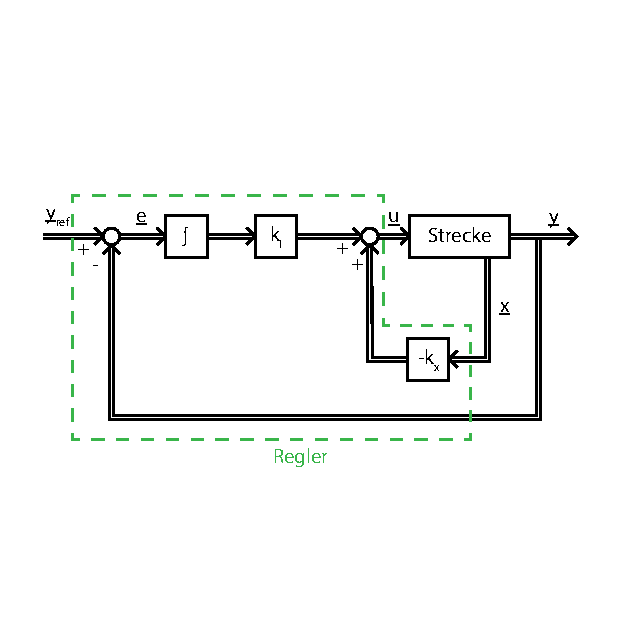
\includegraphics[width=0.7\textwidth]{Bilder/I-Regler.pdf}}
    \caption[Reglerstruktur I-Regelung]{Schematische Darstellung der Reglerstruktur mit I-Regelung}
    \label{fig:Bild11}
\end{figure}

Mit der Definition (\autoref{eq:Gleichung60}) wird das Reglergesetz verändert aufgeschrieben.\\\\
Definition:
\begin{align}\label{eq:Gleichung60}
    \underline{x}_{\mathrm{I}}& :=\int_{0}^t(\underline{y}_{\mathrm{ref}}-\underline{y})d\tau
\end{align}

\clearpage

Einsetzen und Umformen:
\begin{align}
    \underline{u} &= \underline{k}_{\mathrm{I}}\cdot\underline{x}_{\mathrm{I}}-\underline{k}_{\mathrm{x}}\cdot\underline{x} \nonumber \\
    \underline{u} &= -\underline{k}_{\mathrm{x}}\cdot\underline{x}+\underline{k}_{\mathrm{I}}\cdot\underline{x}_{\mathrm{I}} \nonumber\\
    \underline{u} &= -
    \begin{bmatrix}
        \underline{k}_{\mathrm{x}} & -\underline{k}_{\mathrm{I}}
    \end{bmatrix}
    \cdot
    \begin{bmatrix}
        \underline{x} \\
        \underline{x}_{\mathrm{I}}
    \end{bmatrix} \label{eq:Gleichung61} \\
    \underline{\tilde{k}} &= 
    \begin{bmatrix}
        \underline{k}_{\mathrm{x}} & -\underline{k}_{\mathrm{I}}
    \end{bmatrix} \label{eq:Gleichung62}
\end{align}
\newline
Um das erweiterte Zustandsraummodell aufstellen zu können, wird der Zustandsänderungsvektor $\underline{\dot{\tilde{x}}}$ definiert.\\\\
Zustandsänderungsvektor:
\begin{align}
    \underline{\tilde{x}} &=
    \begin{bmatrix}
        \underline{x} \\
        \underline{x}_{\mathrm{I}}
    \end{bmatrix} \nonumber \\
    \underline{\dot{\tilde{x}}} &= 
    \begin{bmatrix}
        \underline{\dot{x}} \\
        \underline{\dot{x}}_{\mathrm{I}}
    \end{bmatrix} \label{eq:Gleichung63}
\end{align}
\newline
Die benötigen Vektoren folgen zu:
\begin{align}
    \underline{\dot{x}} &= \underline{A}\cdot\underline{x}+\underline{B}\cdot\underline{u} \label{eq:Gleichung64}\\
    \underline{\dot{x}}_{\mathrm{I}} &= \frac{d}{dx}\cdot\int_{0}^t(\underline{y}_{\mathrm{ref}}-\underline{y})d\tau = \underline{y}_{\mathrm{ref}}-\underline{y} \nonumber \\
    \underline{\dot{x}}_{\mathrm{I}} &= \underline{y}_{\mathrm{ref}}-\underline{C}\cdot\underline{x} \label{eq:Gleichung65}
\end{align}
\newline
Auf Grundlage der \autoref{eq:Gleichung63} bis \autoref{eq:Gleichung65} folgt das erweiterte Zustandsraummodell zu:\\\\
Erweitertes Zustandsraummodell:
\begin{align}\label{eq:Gleichung66}
    \underline{\dot{\tilde{x}}} &= 
    \begin{bmatrix}
        \underline{A} & \underline{0} \\
        -\underline{C} & \underline{0}
    \end{bmatrix} \cdot \underline{\tilde{x}} +
    \begin{bmatrix}
        \underline{B} \\
        \underline{0}
    \end{bmatrix} \cdot\underline{u} +
    \begin{bmatrix}
        \underline{0} \\
        \underline{I}
    \end{bmatrix} \cdot\underline{y}_{ref}
\end{align}

\clearpage

mit:
\begin{align*}
    \underline{\tilde{A}} &= 
    \begin{bmatrix}
        \underline{A} & \underline{0} \\
        -\underline{C} & \underline{0}
    \end{bmatrix} \quad ; \underline{\tilde{A}}\in\mathbb{R}^{(n+p)x(n+p)}\\
    \underline{\tilde{B}} &= 
    \begin{bmatrix}
        \underline{B} \\
        \underline{0}
    \end{bmatrix}\qquad ; \underline{\tilde{B}}\in\mathbb{R}^{(n+p)x(m)}\\
    \underline{\tilde{B}}_{\mathrm{y}} &= 
    \begin{bmatrix}
        \underline{0} \\
        \underline{I}
    \end{bmatrix}\qquad  ;\underline{\tilde{B}}_{\mathrm{y}}\in\mathbb{R}^{(n+p)x(p)}
\end{align*}
\newline
Die Matrix C wird analog zum Regler mit Referenzwert-Vorsteuerung betrachtet. Mithilfe der Matrizen $\underline{\tilde{A}}$ und $\underline{\tilde{B}}$ werden die Verstärkungskoeffizienten ($\underline{k}_{\mathrm{x}}$ und $\underline{k}_{\mathrm{I}}$) analog zu \autoref{sec:Ackermann-Formel} berechnet. Die Polstellen des Reglers werden entsprechend festgelegt (\autoref{eq:Gleichung67}).
\begin{align}\label{eq:Gleichung67}
    \underline{s}_{\mathrm{P}} &= 
    \begin{bmatrix}
        -3.2 & -3.2 & -3.2 & -3.2 & -3.2
    \end{bmatrix}
\end{align}
\newline
Die Länge des Vektors folgt auf Grundlage der Größe der Matrix $\underline{\tilde{A}}$. Die Lage der Polstellen ist in \autoref{fig:Bild12} dargestellt.

\begin{figure}[H]
    \centering
    \fbox{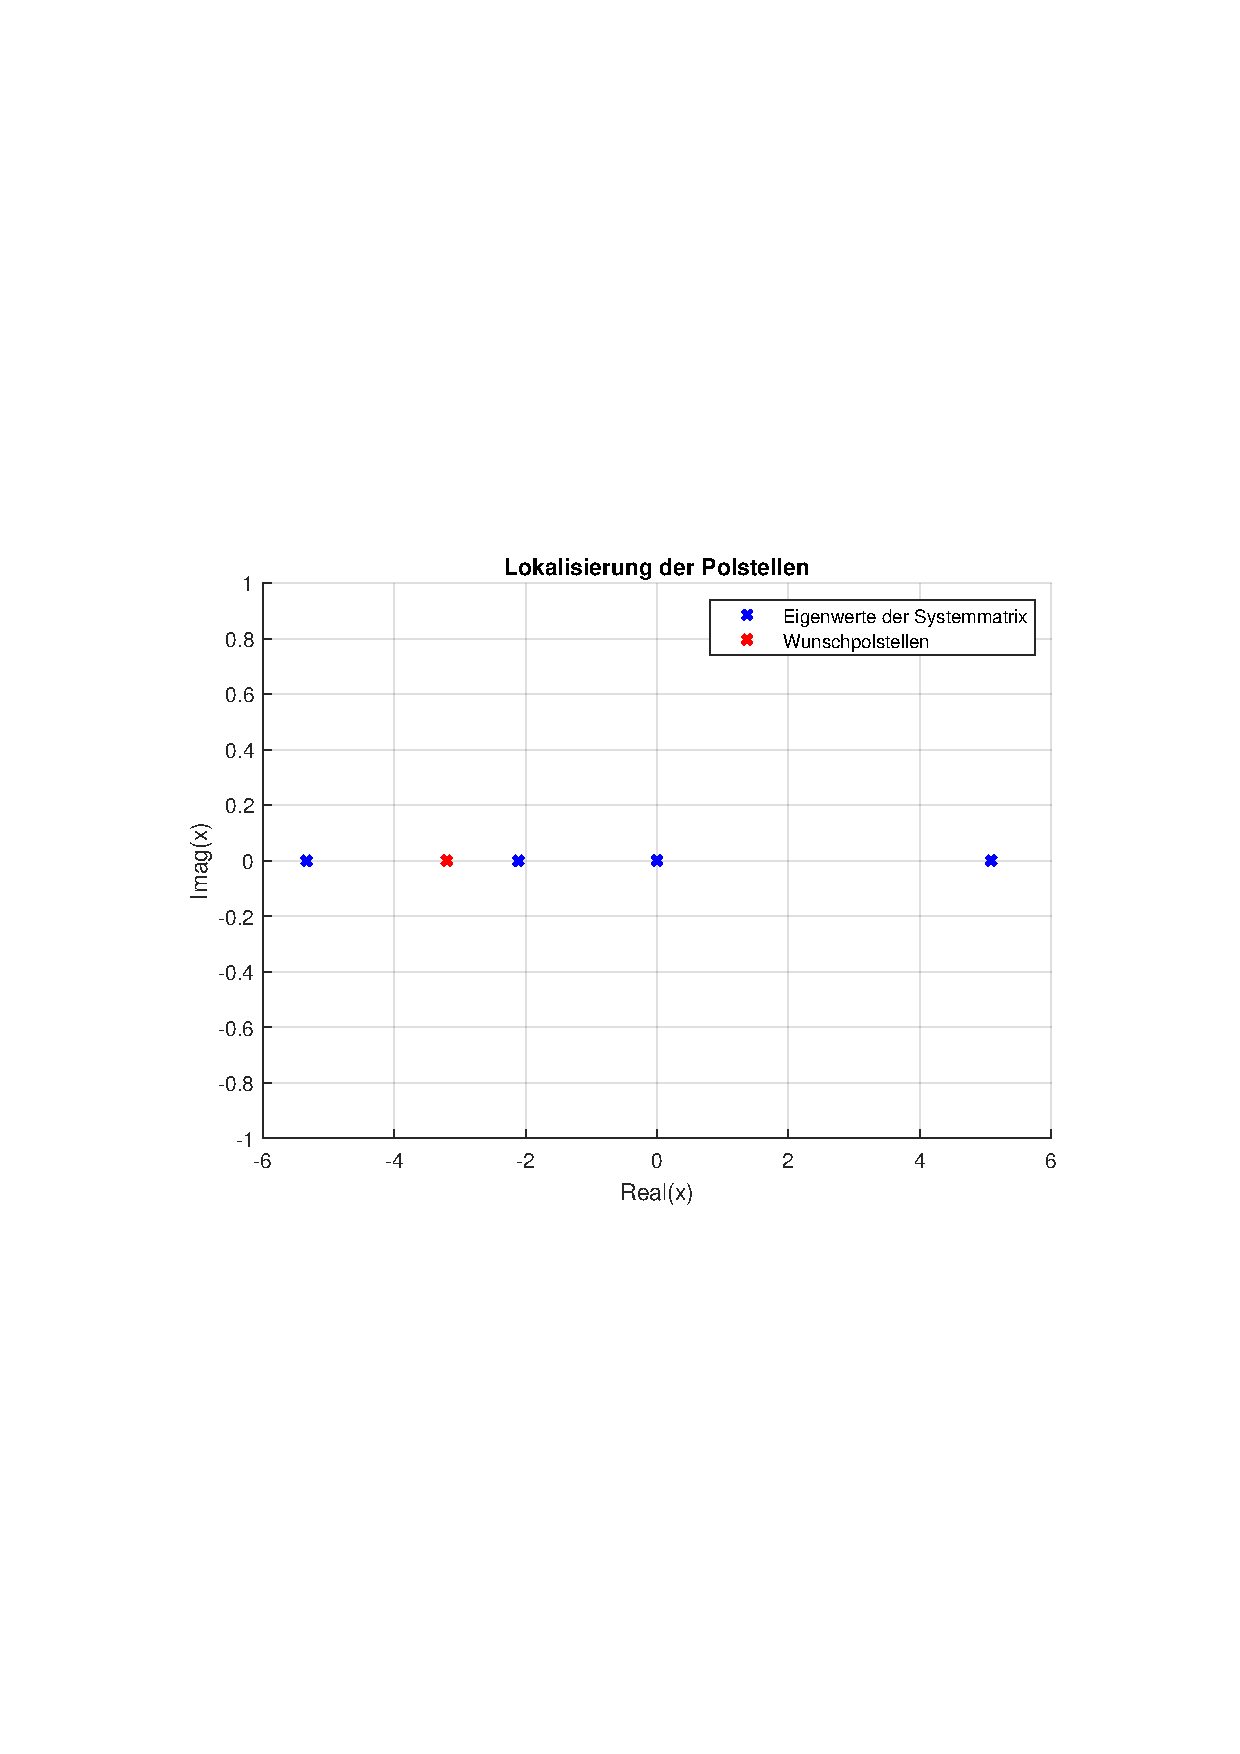
\includegraphics[width=0.75\textwidth]{Bilder/Polstellen_I_Regelung.pdf}}
    \caption[Polstellenlage I-Regelung]{Polstellenlage des Systems mit I-Regelung}
    \label{fig:Bild12}
\end{figure}

Die $\underline{\tilde{k}}$-Matrix resultiert zu:
\begin{align}\label{eq:Gleichung68}
    \underline{\tilde{k}} &= 
    \begin{bmatrix}
        -180.9111 & -35.8968 & -64.1713 & -48.8165 & 41.0452
    \end{bmatrix}
\end{align}
\newline
Gemäß \autoref{eq:Gleichung62} folgen die Verstärkungskoeffizienten wie nachfolgend gezeigt:\\\\
Zustandsrückführungskoeffizienten:
\begin{align}\label{eq:Gleichung69}
    \underline{k}_{\mathrm{x}} &= 
    \begin{bmatrix}
        -180.9111 & -35.8968 & -64.1713 & -48.8165
    \end{bmatrix}
\end{align}
\newline
I-Verstärkungskoeffizienten:
\begin{align}\label{eq:Gleichung70}
    \underline{k}_{\mathrm{I}} &= [-41.0452]
\end{align}